\documentclass{article}
\usepackage{amsmath}
\usepackage{amssymb}
\usepackage{graphicx}
\usepackage{hyperref}
\usepackage[version=4]{mhchem}

\title{Problem 6}
\date{}

\begin{document}
\maketitle

\section*{Problem}
(AMC) Two congruent \(30^{\circ}-60^{\circ}-90^{\circ}\) triangles are placed so that they overlap partly and their hypotenuses coincide. If the hypotenuse of each triangle is 12 , the area common to both triangles is\\
(A) \(6 \sqrt{3}\)\\
(B) \(8 \sqrt{3}\)\\
(C) \(9 \sqrt{3}\)\\
(D) \(12 \sqrt{3}\)\\
(E) 24\\
\centering
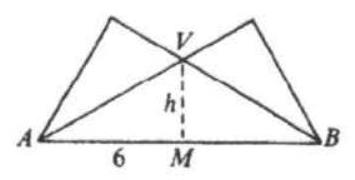
\includegraphics[width=\textwidth]{images/089.jpg}

\section*{Solution}
Solution not available.

\end{document}
